% GENERATED by thumbnail/build_thumbnail.py -- do not edit.
% Sources: results/phase4/thesis_numbers.json, agr/budget.py,
%          results/phase4/test_webqsp.json
\documentclass[border=0pt]{standalone}
\usepackage[T1]{fontenc}
\usepackage[scaled=0.92]{helvet}
\renewcommand{\familydefault}{\sfdefault}
% A card is read at a glance; a word broken across two lines in a 34mm
% node costs more than the ragged edge it saves.
\hyphenpenalty=10000 \exhyphenpenalty=10000 \tolerance=3000
\usepackage{tikz}
\usetikzlibrary{arrows.meta, positioning, backgrounds, fit, calc}

% The deck's palette, which is Okabe-Ito: colour is semantic and every
% distinction is also carried by shape or position, so a greyscale
% reproduction of this card loses nothing.
\definecolor{agrdark}{RGB}{28,54,78}
\definecolor{agraccent}{RGB}{176,58,46}
\definecolor{agrgrey}{RGB}{110,110,110}
\definecolor{agrNode}{HTML}{0072B2}
\definecolor{agrSup}{HTML}{009E73}
\definecolor{agrUns}{HTML}{D55E00}
\definecolor{agrPaper}{HTML}{FBFCFD}

\begin{document}
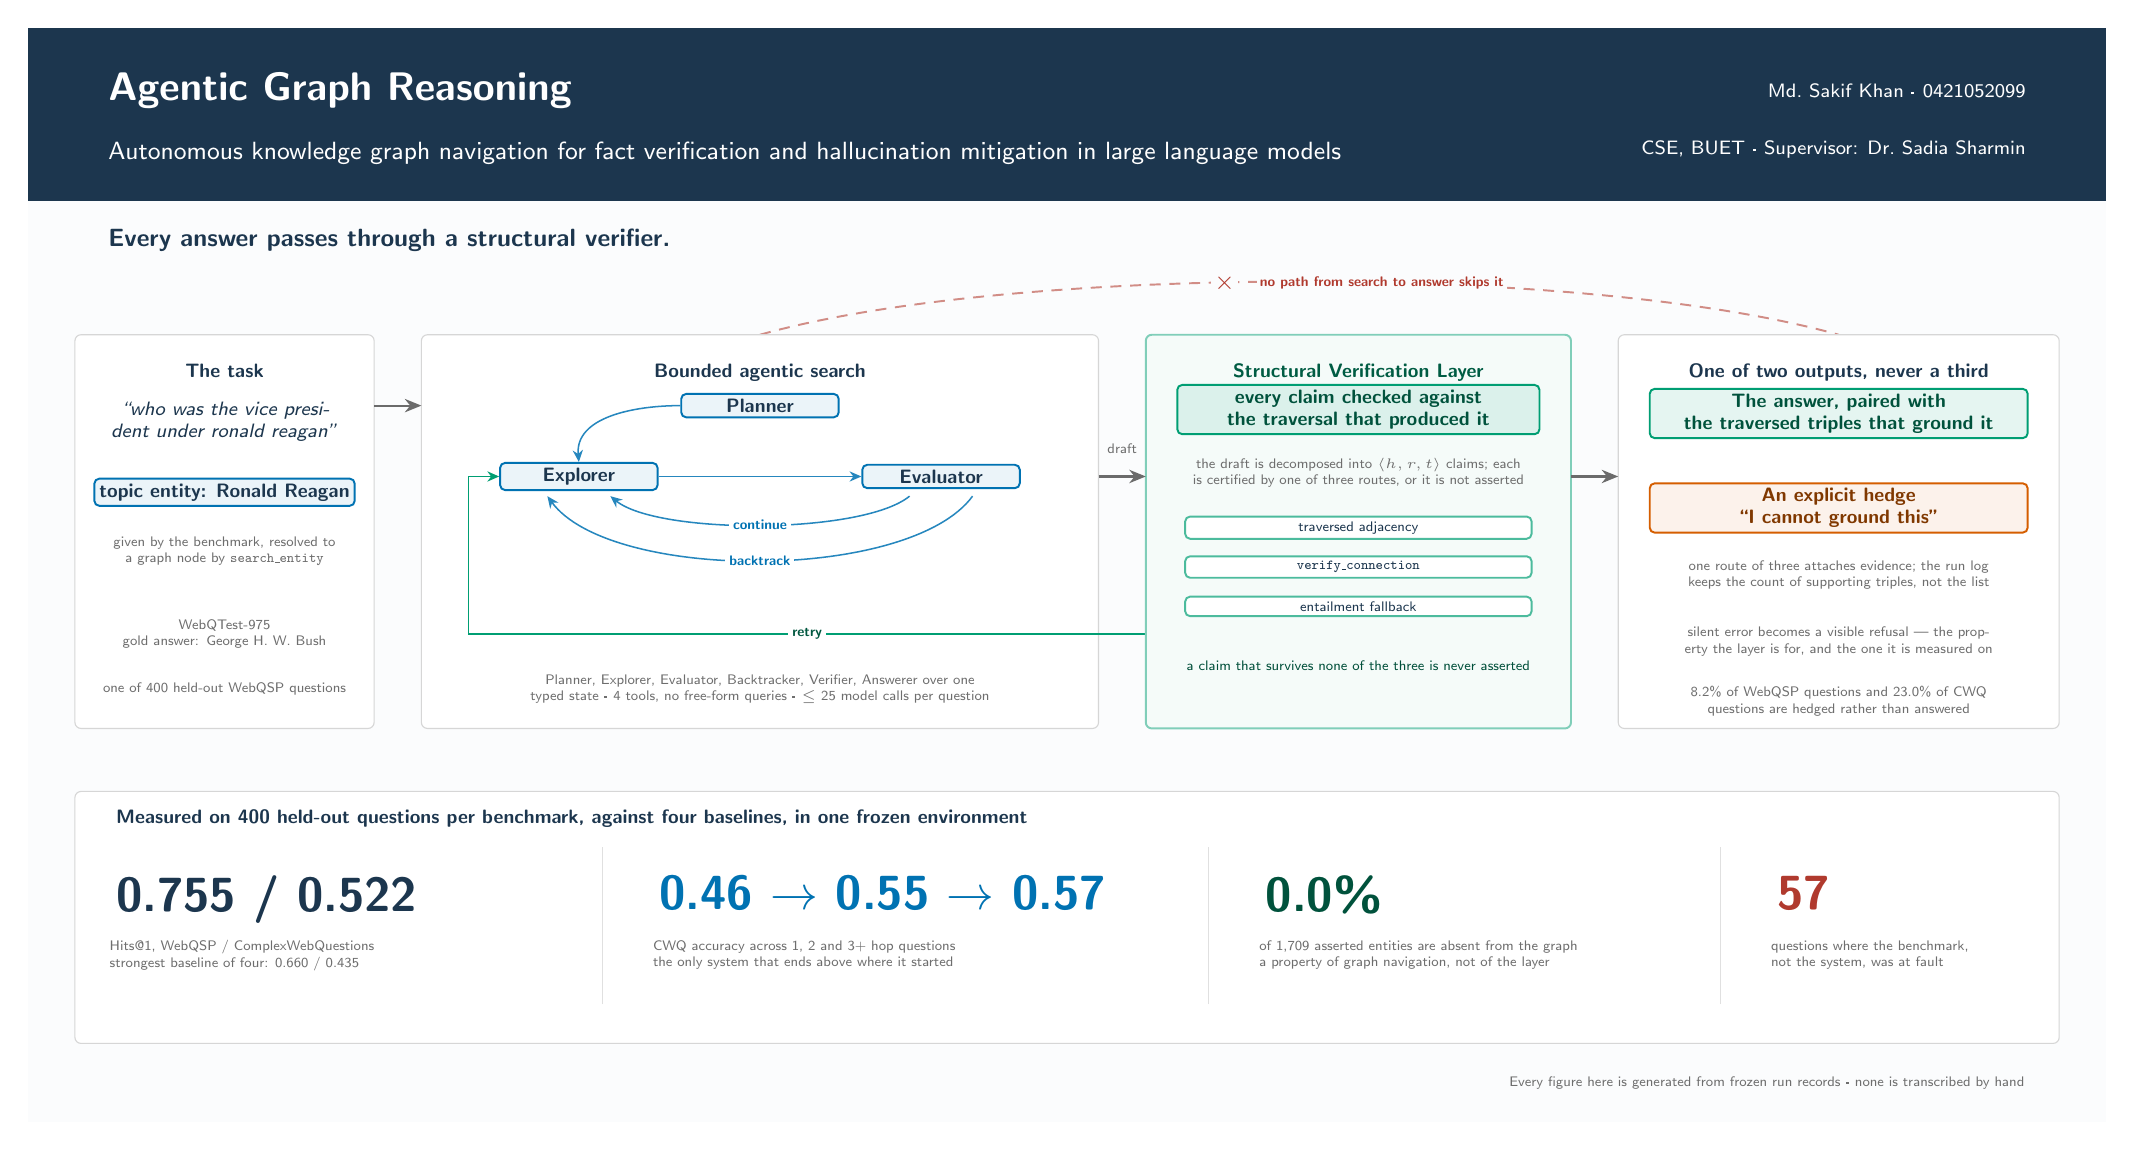
\begin{tikzpicture}[
    x=1mm, y=1mm,
    stage/.style={draw=black!16, rounded corners=2.2pt, fill=white,
                  line width=0.4pt},
    head/.style={font=\scriptsize\bfseries, text=agrdark},
    node/.style={draw=agrNode, line width=0.7pt, rounded corners=1.8pt,
                 fill=agrNode!8, align=center, font=\scriptsize\bfseries,
                 inner sep=1.8pt, text=agrdark},
    flow/.style={-{Stealth[length=2.1mm,width=1.7mm]}, line width=0.8pt,
                 draw=black!58},
    thinflow/.style={-{Stealth[length=1.5mm,width=1.3mm]}, line width=0.55pt,
                     draw=agrNode!85},
    lbl/.style={font=\tiny, text=agrgrey, inner sep=1pt},
    cyc/.style={font=\tiny\bfseries, text=agrNode, inner sep=1.4pt,
                fill=white}]

\fill[agrPaper] (0,4) rectangle (264,143);

% ================= title band ======================================
\fill[agrdark] (0,121) rectangle (264,143);
\node[anchor=west, text=white, font=\Large\bfseries] at (9,135)
  {Agentic Graph Reasoning};
\node[anchor=west, text=white!76, font=\small] at (9,127)
  {Autonomous knowledge graph navigation for fact verification and
   hallucination mitigation in large language models};
\node[anchor=east, text=white!62, font=\scriptsize] at (255,135)
  {Md.\ Sakif Khan \textperiodcentered\ 0421052099};
\node[anchor=east, text=white!62, font=\scriptsize] at (255,127.5)
  {CSE, BUET \textperiodcentered\ Supervisor: Dr.\ Sadia Sharmin};

% ================= the claim, and the route that does not exist ====
\node[anchor=west, font=\small\bfseries, text=agrdark] at (9,116)
  {Every answer passes through a structural verifier.};
\draw[dashed, dash pattern=on 1.4mm off 1.1mm, line width=0.7pt,
      draw=agraccent!58]
  (93,104) .. controls (125,113) and (198,113) .. (230,104);
\node[font=\small\bfseries, text=agraccent, fill=agrPaper,
      inner sep=1.4pt] at (152,110.6) {$\times$};
% The label sits on the arc, so it carries the page colour: without it
% the dashes run through the words and read as a strikethrough.
\node[font=\tiny\bfseries, text=agraccent, anchor=west, fill=agrPaper,
      inner sep=1.2pt] at (156,110.6)
  {no path from search to answer skips it};

% ================= 1. question =====================================
\node[stage, minimum width=38mm, minimum height=50mm] (qbox) at (25,79) {};
\node[head, anchor=north] at (25,101.5) {The task};
\node[font=\scriptsize\itshape, text=agrdark, align=center,
      text width=34mm] at (25,93) {``who was the vice president under ronald reagan''};
\node[node, minimum width=30mm] (topic) at (25,84)
  {topic entity: Ronald Reagan};
\node[lbl, align=center, text width=34mm] at (25,76.5)
  {given by the benchmark, resolved to a graph node by
   \texttt{search\_entity}};
\node[lbl, align=center, text width=34mm] at (25,66)
  {WebQTest-975\\ gold answer: George H. W. Bush};
\node[lbl, align=center, text width=34mm] at (25,59)
  {one of 400 held-out WebQSP questions};

% ================= 2. bounded agentic search =======================
\node[stage, minimum width=86mm, minimum height=50mm] (sbox) at (93,79) {};
\node[head, anchor=north] at (93,101.5) {Bounded agentic search};

\node[node, minimum width=20mm] (plan) at (93,95) {Planner};
\node[node, minimum width=20mm] (expl) at (70,86) {Explorer};
\node[node, minimum width=20mm] (eval) at (116,86) {Evaluator};

\draw[thinflow] (plan.west) to[out=180,in=95] (expl.north);
\draw[thinflow] (expl.east) -- (eval.west);

% Three cycles -- continue, backtrack, retry -- which is what the thesis
% figure draws and what the deck says. Nested arcs into the Explorer are
% what three cycles look like; the Backtracker is named in the caption
% rather than drawn, because the card needs the cycles, not every node.
\draw[thinflow] (112,83.5) .. controls (106,78.6) and (80,78.6)
  .. node[cyc, pos=0.5] {continue} (74,83.5);
\draw[thinflow] (120,83.5) .. controls (112,72.6) and (74,72.6)
  .. node[cyc, pos=0.5] {backtrack} (66,83.5);
\draw[thinflow, draw=agrSup] (142,66) -- (56,66) -- (56,86)
  -- (expl.west);
\node[cyc, text=agrSup!55!black] at (99,66) {retry};

\node[lbl, align=center, text width=80mm] at (93,59)
  {Planner, Explorer, Evaluator, Backtracker, Verifier, Answerer over one
   typed state \textperiodcentered\ 4 tools, no free-form queries
   \textperiodcentered\ $\leq$ 25 model calls per question};

% ================= 3. the verifier =================================
\node[stage, minimum width=54mm, minimum height=50mm, draw=agrSup!50,
      fill=agrSup!4, line width=0.7pt] (vbox) at (169,79) {};
\node[head, anchor=north, text=agrSup!58!black] at (169,101.5)
  {Structural Verification Layer};
\node[node, minimum width=46mm, draw=agrSup, fill=agrSup!14,
      text=agrSup!52!black] (ver) at (169,94.5)
  {every claim checked against\\ the traversal that produced it};
\node[lbl, align=center, text width=50mm] at (169,86.5)
  {the draft is decomposed into $\langle h,r,t \rangle$ claims; each is
   certified by one of three routes, or it is not asserted};
\node[node, minimum width=44mm, draw=agrSup!70, fill=white, font=\tiny,
      text=agrdark] at (169,79.5) {traversed adjacency};
\node[node, minimum width=44mm, draw=agrSup!70, fill=white, font=\tiny,
      text=agrdark] at (169,74.5) {\texttt{verify\_connection}};
\node[node, minimum width=44mm, draw=agrSup!70, fill=white, font=\tiny,
      text=agrdark] at (169,69.5) {entailment fallback};
\node[lbl, align=center, text width=50mm, text=agrSup!50!black]
  at (169,62) {a claim that survives none of the three is never asserted};

% ================= 4. output =======================================
\node[stage, minimum width=56mm, minimum height=50mm] (obox) at (230,79) {};
\node[head, anchor=north] at (230,101.5) {One of two outputs, never a third};
\node[node, minimum width=48mm, draw=agrSup, fill=agrSup!10,
      text=agrSup!52!black] (ans) at (230,94)
  {\textbf{The answer}, paired with\\ the traversed triples that ground it};
\node[node, minimum width=48mm, draw=agrUns, fill=agrUns!8,
      text=agrUns!60!black] (hedge) at (230,82)
  {\textbf{An explicit hedge}\\ ``I cannot ground this''};
% The two bounds, on the card that makes the claim. A long document can
% claim the contract in section 1 and withdraw it in section 6 because
% section 6 is always there to be read; an event card has no section 6.
\node[lbl, align=center, text width=50mm] at (230,73.5)
  {one route of three attaches evidence; the run log keeps the count of
   supporting triples, not the list};
\node[lbl, align=center, text width=50mm] at (230,65)
  {silent error becomes a visible refusal --- the property the layer is
   for, and the one it is measured on};
% hedge_pct is a share of QUESTIONS (scripts/score_test.py counts
% `not pred` over per-question rows), and a hedge is by definition not an
% answer, so "of answers" contradicted itself.
\node[lbl, align=center, text width=50mm] at (230,57.5)
  {8.2\% of WebQSP questions and 23.0\% of CWQ questions
   are hedged rather than answered};

% ================= the spine =======================================
\draw[flow] (44,95) -- (50,95);
\draw[flow] (136,86) -- (142,86);
\node[lbl, fill=agrPaper, inner sep=1.2pt] at (139,89.5) {draft};
\draw[flow] (196,86) -- (202,86);

% ================= results strip ===================================
\node[stage, minimum width=252mm, minimum height=32mm] at (132,30) {};
\node[anchor=west, head] at (10,42.5)
  {Measured on 400 held-out questions per benchmark, against four
   baselines, in one frozen environment};

\node[anchor=north west, font=\LARGE\bfseries, text=agrdark]
  at (10,36.5) {0.755 / 0.522};
\node[anchor=north west, lbl, align=left] at (10,27.5)
  {Hits@1, WebQSP / ComplexWebQuestions\\
   strongest baseline of four: 0.660 / 0.435};

\draw[draw=black!12] (73,19) -- (73,39);
\node[anchor=north west, font=\LARGE\bfseries, text=agrNode]
  at (79,36.5) {0.46 $\rightarrow$ 0.55 $\rightarrow$ 0.57};
\node[anchor=north west, lbl, align=left] at (79,27.5)
  {CWQ accuracy across 1, 2 and 3+ hop questions\\
   the only system that ends above where it started};

\draw[draw=black!12] (150,19) -- (150,39);
\node[anchor=north west, font=\LARGE\bfseries, text=agrSup!52!black]
  at (156,36.5) {0.0\%};
\node[anchor=north west, lbl, align=left] at (156,27.5)
  {of 1,709 asserted entities are absent from the graph\\
   a property of graph navigation, not of the layer};

\draw[draw=black!12] (215,19) -- (215,39);
\node[anchor=north west, font=\LARGE\bfseries, text=agraccent]
  at (221,36.5) {57};
\node[anchor=north west, lbl, align=left] at (221,27.5)
  {questions where the benchmark,\\ not the system, was at fault};

\node[anchor=east, lbl] at (254,9)
  {Every figure here is generated from frozen run records
   \textperiodcentered\ none is transcribed by hand};
\end{tikzpicture}
\end{document}
